\documentclass{scrartcl}
\usepackage{graphicx}  % required for inserting images

% for cyrillic and Bulgarian language
\usepackage[utf8]{inputenc}
\usepackage[T2A]{fontenc}
\usepackage[bulgarian]{babel}

% math packages
\usepackage{amsmath}
\usepackage{float}
\usepackage{amsfonts}
\usepackage{amssymb}
\usepackage{amsthm}
\usepackage{cancel}

\usepackage{ragged2e}  % adds FlushLeft
\usepackage{booktabs}
\usepackage{tabularx}

\usepackage{listings}
\usepackage{xcolor}

\definecolor{codegreen}{rgb}{0,0.6,0}
\definecolor{codegray}{rgb}{0.5,0.5,0.5}
\definecolor{codepurple}{rgb}{0.58,0,0.82}
\definecolor{backcolour}{rgb}{0.95,0.95,0.92}

\lstdefinestyle{mystyle}{
    %caption=Example C++,
    label={lst:listing-cpp},
    language=C++,
    backgroundcolor=\color{backcolour},   
    commentstyle=\color{codegreen},
    keywordstyle=\color{magenta},
    numberstyle=\tiny\color{codegray},
    stringstyle=\color{codepurple},
    basicstyle=\ttfamily\footnotesize,
    breakatwhitespace=false,         
    breaklines=true,                 
    keepspaces=true,                 
    numbers=left,       
    numbersep=5pt,                  
    showspaces=false,                
    showstringspaces=false,
    showtabs=false,                  
    tabsize=2,
}
\lstset{style=mystyle}

\usepackage[colorlinks=true, linkcolor=blue, urlcolor=cyan]{hyperref}

\newtheorem{theorem}{Теорема}
\newtheorem{definition}{Дефиниция}

\title{Проектиране и интегриране на софтуерни системи}
\author{Ивайло Андреев + gemini 3 Flash, Claude Sonnet 4.6}
\date{22 юни 2026}

\begin{document}
\maketitle

\tableofcontents

\newpage

\begin{FlushLeft}

\section{Характеристики на разпределените софтуерни системи}

\subsection{Дефиниции}
В съвременното софтуерно инженерство (по Таненбаум и стандарта IEEE) са утвърдени следните две основни дефиниции за разпределена софтуерна система:
\begin{itemize}
    \item Група от независими компютри, която за крайния потребител изглежда и се възприема като една единствена, цялостна система.
    \item Система, в която хардуерни или софтуерни компоненти, намиращи се на мрежови компютри (възли), комуникират помежду си и координират своите действия изцяло и единствено чрез изпращане и обмен на съобщения.
\end{itemize}

\subsection{Основни характеристики на системите}
Разпределените системи се проектират с цел постигане на следните пет ключови софтуерни архитектурни качества:
\begin{enumerate}
    \item \textbf{Свързаност и комуникация:} Възможност за безпрепятствен обмен на ресурси и данни между отдалечените възли.
    \item \textbf{Хетерогенност:} Способност на системата да работи интегрирано, независимо от различията в хардуера, операционните системи, мрежовите протоколи и езиците за програмиране.
    \item \textbf{Мащабируемост (Scalability):} Капацитет на системата да реагира адекватно при значително нарастване на натоварването. Реализира се по два начина: \textbf{хоризонтално мащабиране} (\textit{horizontal scaling}) — добавяне на нови възли към системата, и \textbf{вертикално мащабиране} (\textit{vertical scaling}) — увеличаване на ресурсите (CPU, RAM) на съществуващите възли.
    \item \textbf{Отказоустойчивост при частични откази:} Способност на архитектурата да продължи стабилното си функциониране, дори когато определени възли или комуникационни канали отпаднат.
    \item \textbf{Сигурност и надеждност:} Защита на данните и транзакциите при пренос по публични или споделени мрежи.
\end{enumerate}

\subsection{Видове разпределени системи}
Разпределените софтуерни системи се класифицират в три основни категории:

\subsubsection{1. Разпределени изчислителни системи (Distributed Computing Systems)}
Използват се за тежки изчислителни задачи, изискващи изключително висока производителност. Разделят се на:
\begin{itemize}
    \item \textbf{Клъстери (Cluster Computing):} Силно свързани (\textit{tightly coupled}) системи. Възлите са идентични като хардуер и операционна система, физически близо един до друг, свързани в една високоскоростна локална мрежа, като една програма работи паралелно върху всички тях.
    \item \textbf{Гридове (Grid Computing):} Слабо свързани (\textit{loosely coupled}) хетерогенни системи, при които хардуерът, операционните системи и мрежите на отделните възли се различават драстично. Възлите често са географски и физически силно отдалечени един от друг.
\end{itemize}

\subsubsection{2. Разпределени информационни системи (Distributed Information Systems)}
Проектирани са с цел интеграция и свързване на множество разнообразни приложения, които си комуникират по мрежата, но първоначално могат да бъдат оперативно несъвместими. Интеграцията се извършва на няколко нива:
\begin{itemize}
    \item \textbf{Клиент-Сървър (Client-Server):} На по-ниско технологично ниво клиентите групират и изпращат заявки към сървъра, които се изпълняват по "атомарен" начин (в тяхната цялост).
    \item \textbf{Peer-to-Peer (P2P):} На по-високо ниво, където всяко приложение (възел) действа едновременно като клиент и като сървър, позволявайки директна комуникация помежду им без централен посредник.
\end{itemize}

\subsubsection{3. Широкоразпространени / Повсеместни разпределени системи (Pervasive Distributed Systems)}
За разлика от стабилните промишлени системи, тези системи по дефиниция са изключително нестабилни. Това се налага поради масовото навлизане на мобилни, преносими и вградени (embedded) изчислителни системи.
\begin{itemize}
    \item Възлите в тези системи са малки, мобилни, захранват се от батерии и използват безжични комуникации.
    \item Характеризират се с ад-хок свързване и пълна липса на нужда от непрекъснат човешки надзор или администрация. Примери за това са умните коли, авиационните системи и IoT сензорните мрежи.
\end{itemize}

\subsection{Архитектурни тенденции}
\begin{itemize}
    \item Масово навлизане на повсеместната изчислителност и IoT уреди (смарт часовници, коли, сензори).
    \item Постоянно разширяване на Интернет като глобална разпределена мрежа и драстично нарастване на търсенето на мултимедийни и стрийминг услуги (Webcasting).
    \item Доминиране на разпределени системи "по заявка" (\textit{on-demand}) и Облачни изчисления (\textit{Cloud Computing} като AWS, Azure, Google Cloud).
\end{itemize}

\section{Междупроцесна комуникация (Inter-Process Communication - IPC)}

Комуникацията между процесите в разпределена среда се базира на обмен на съобщения. Ядрото на операционната система предоставя нисконивови механизми за IPC като \textbf{опашки от съобщения (message queues)}, \textbf{семафори} и \textbf{споделена памет (shared memory)}.

В разпределените системи тези IPC механизми рядко се използват директно от програмистите. Вместо това те се капсулират от \textbf{междинен софтуер (middleware)}, който предоставя високо ниво на абстракция чрез интерфейси. Middleware скрива хетерогенността на хардуера, операционните системи и мрежата, като осигурява стандартизирана комуникация, прозрачност и координация между разпределените компоненти.

Основни функции на middleware:
\begin{itemize}
    \item Именуване и адресиране на компоненти
    \item Маршалинг/демаршалинг на данни (сериализация)
    \item Управление на транзакции
    \item Сигурност и автентикация
    \item Балансиране на натоварването
\end{itemize}

Важна част от този middleware е \textit{message-passing} механизмът за комуникация без споделена памет.

Комуникацията се разделя на два типа:
\begin{itemize}
    \item \textbf{Connection-oriented:} Изисква изграждането на изричен, специален канал за комуникация между процесите.
    \item \textbf{Message-oriented:} Преизползва вече съществуващи мрежови канали за изпращане на независими пакети данни.
\end{itemize}

\subsection{Отдалечено извикване}
Отдалечените извиквания позволяват на процес А да използва функционалност, намираща се в процес В, по напълно "прозрачен" за себе си начин — маскирайки факта, че В е външен процес, намиращ се на друга машина. Имплементира се чрез две основни технологии:

\subsubsection{1. Remote Procedure Call (RPC)}
RPC позволява извикване на процедура на отдалечен възел, прозрачно за извикващия — като локална функция. Middleware се грижи за сериализацията на параметрите (\textbf{маршалинг}) и десериализацията на резултата (\textbf{демаршалинг}).

RPC се базира на предоставянето на интерфейси, които специфицират процедурите, предлагани от отдалечения процес, скривайки изцяло имплементацията им. Интерфейсите се описват чрез \textbf{IDL (Interface Definition Language)}, чиято цел е да позволи процедура, написана на един език, да бъде извикана от клиент, написан на съвсем различен език. Модерна имплементация на този подход е протоколът \textbf{gRPC} на Google (базиран на HTTP/2 и Protocol Buffers).

RPC дефинира три основни семантики на извикване при възникване на грешки в мрежата:
\begin{itemize}
    \item \textbf{maybe:} Процедурата се изпълнява веднъж или изобщо не се изпълнява, като клиентът не получава потвърждение.
    \item \textbf{at-least-once:} Клиентът гарантирано получава резултат само ако процедурата се е изпълнила поне веднъж (възможни са повторения при препредаване на заявката).
    \item \textbf{at-most-once:} Клиентът знае, че процедурата се е изпълнила най-много веднъж, елиминирайки риска от дублиране на операции.
    \item \textbf{exactly-once:} Теоретично гарантира точно едно изпълнение, но е изключително трудно постижимо на практика в ненадеждни мрежи, тъй като изисква синхронизация между изпращача и получателя.
\end{itemize}

\subsubsection{2. Remote Method Invocation (RMI)}
RMI е обектно-ориентираният аналог на RPC за Java. Позволява извикване на методи на отдалечени обекти. Използва \textbf{stub} (клиентска страна) и \textbf{skeleton} (сървърна страна) за прозрачна комуникация.
\begin{itemize}
    \item \textbf{Прилики с RPC:} Поддържа строг модел на програмиране с интерфейси, базира се на нисконивовия протокол заявка-отговор и осигурява високо ниво на прозрачност.
    \item \textbf{Разлики от RPC:} Поддържа изцяло обектно-ориентираната парадигма и позволява предаването на реални референции към обекти като параметри на методите.
\end{itemize}

\begin{figure}[H]
    \centering
    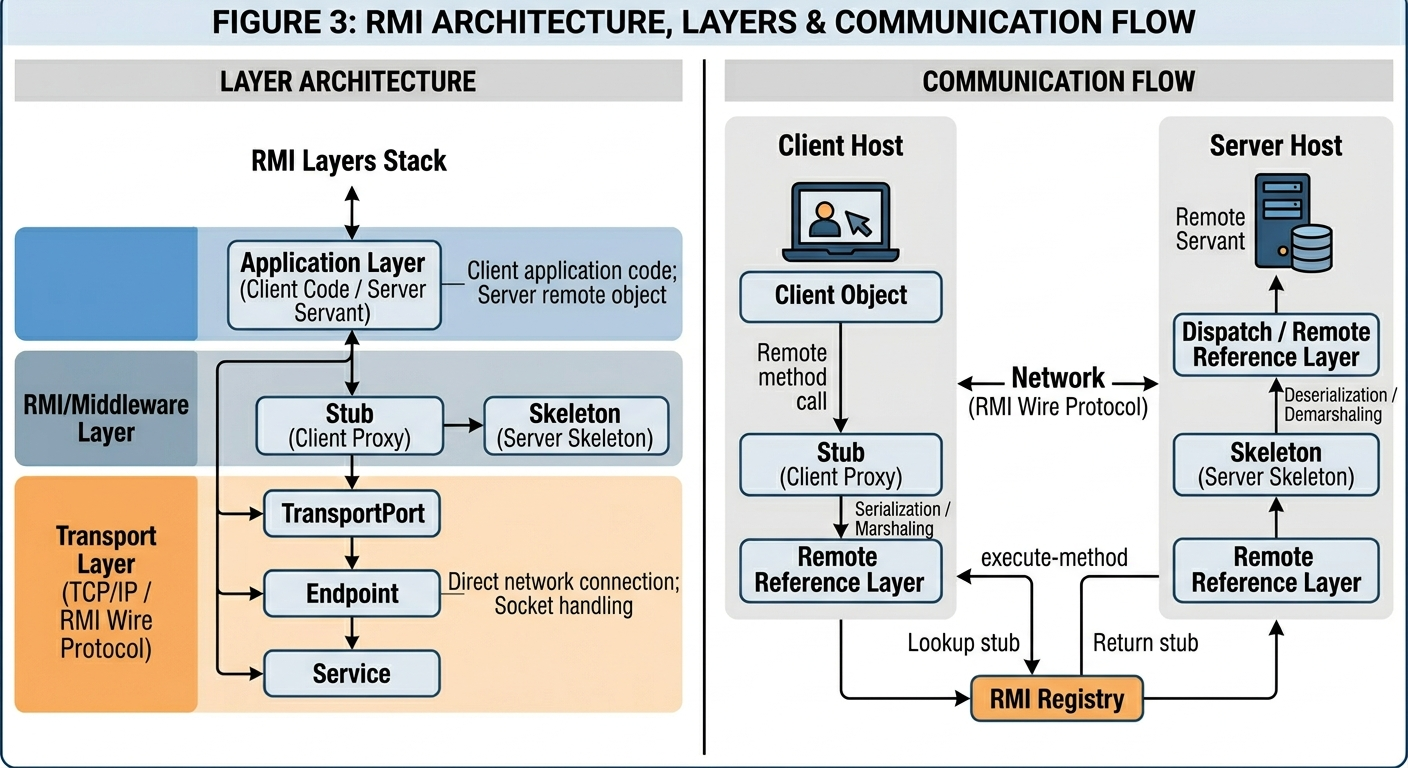
\includegraphics[width=0.8\textwidth]{pictures/rmi.png}
    \caption{Архитектурен модел, слоеве и динамичен поток на RMI комуникация}
    \label{fig:rmi}
\end{figure}

На Фиг. \ref{fig:rmi} са илюстрирани два взаимно свързани аспекта на технологията: \textbf{слоевата архитектура} (вляво) и \textbf{динамичният комуникационен поток} (вдясно). 

Ключовият архитектурен елемент в динамичния модел е \textbf{RMI Registry} — разпределена директорийна услуга (наименуващ регистър), работеща на специфичен порт на сървъра. Ролята му е да служи като посредник при първоначалното свързване. Процесът протича на три етапа:
\begin{enumerate}
    \item \textbf{Регистрация (Bind):} Сървърният обект (Remote Servant) се регистрира в RMI Registry под уникално текстово име.
    \item \textbf{Търсене (Lookup):} Клиентът изпраща заявка към RMI Registry по името на услугата и получава обратно локално прокси референция (\textit{Stub}).
    \item \textbf{Директна комуникация:} След като клиентът притежава \textit{Stub}-а, RMI Registry излиза от комуникационния канал. Извикването на метод се маршализира от Remote Reference слоя на клиента, пренася се по мрежата чрез специфичния RMI Wire протокол и се демаршализира от слоевете на сървъра (Skeleton), задействайки реалния Servant обект.
\end{enumerate}

Имплементационната архитектура на RMI се състои от следните задължителни модули (виж Фиг. \ref{fig:rmi}):
\begin{itemize}
    \item \textbf{Клиент (Client Application):} Инициира извикването на метода.
    \item \textbf{RMI Слой:} Съдържа Client Proxy (Stub), Servant Skeleton, Remote Reference Module (за маршализация на данните) и Dispatcher.
    \item \textbf{Маршализация/Демаршализация:} Процесите на сериализация/десериализация на обектите при предаване по мрежата.
    \item \textbf{Сървър (Servant/Dispatcher):} Реалната инстанция на отдалечения обект.
    \item \textbf{Транспортен слой:} Управлява физическата TCP/IP връзка по мрежата.
\end{itemize}

\subsubsection{3. CORBA (Common Object Request Broker Architecture)}
CORBA е платформено-независим стандарт на OMG за комуникация между разпределени обекти. Той решава хетерогенността, като позволява на компоненти, написани на различни езици (C++, Java, Python), да комуникират прозрачно чрез IDL-дефинирани интерфейси.

Ключови компоненти на CORBA:
\begin{itemize}
    \item \textbf{ORB (Object Request Broker):} Посредникът, който маршрутизира заявките между обектите.
    \item \textbf{IDL (Interface Definition Language):} Езиково-неутрален език за описание на интерфейсите.
    \item \textbf{IIOP (Internet Inter-ORB Protocol):} Протоколът за комуникация между ORB-овете.
    \item \textbf{Naming Service:} Регистър за именуване на обекти (аналог на DNS).
\end{itemize}

\subsection{Мултикаст (Multicast)}
Мултикастът е метод за едновременно изпращане на едно съобщение от един изпращач до дефинирана група от много получатели в мрежата. Мрежовата топология на тези групи се оформя като \textbf{дърво} (директен достъп) или \textbf{mesh} (наличие на множество алтернативни пътища).

Тъй като рутерите на приложно ниво не се борят за междинни възли, рутирането се оптимизира чрез епидемични алгоритми — \textbf{Gossip-Based Data Dissemination}. Подобно на биологичен вирус, всеки възел, който притежава информацията ("заразен" възел), я предава автономно на своите съседни възли. Изтриването на информация в такива децентрализирани епидемични мрежи е трудно, поради което се симулира "изтриване чрез модификация" (death certificates).

\section{Разпределени обекти и компоненти}

\subsection{Разпределени обекти}
При този дизайн архитектурните единици са разпределени обекти, които комуникират чрез RMI или механизма на разпределените събития. Те осигуряват капсулация и силна абстракция на данните. 

\textbf{Основни дефекти и проблеми на обектния подход:}
\begin{itemize}
    \item Интерфейсите на обектите описват само методите, но не дефинират изрично контекстните зависимости на имплементацията им.
    \item Програмистите са принудени ръчно да имплементират и управляват сложни системни детайли като конкурентност, нисконивова сигурност и обработка на мрежови грешки.
    \item Липсва автоматизирана (\textit{out-of-the-box}) поддръжка за управление на жизнения цикъл и сложни конфигурации от обекти.
\end{itemize}

\subsection{Разпределени компоненти}
Проблемите на обектите налагат прехода към парадигмата на разпределените компоненти. \textbf{Софтуерният компонент} е независима градивна единица, която задължително дефинира както интерфейсите, които предоставя (\textit{provided interfaces}), така и своите \textbf{експлицитни контекстни зависимости} (\textit{required interfaces}).
Инфраструктурата на компонентите се управлява автоматизирано от контейнери, които поемат сигурността и конкурентността. Индустриални стандарти за разпределени компоненти са \textbf{Enterprise Java Beans (EJB)} и архитектурата \textbf{CORBA}.

\section{Уеб услуги (Web Services)}

\subsection{Дефиниции и архитектурни цели}
\begin{itemize}
    \item \textbf{Интерфейс на уеб услуга:} Колекция от операции, изложени и достъпни по стандартизиран начин през Интернет, които се имплементират от хетерогенни ресурси (програми, бази данни).
    \item \textbf{Транспорт:} Уеб услугите се достъпват предимно чрез приложния протокол \textbf{HTTP}.
    \item \textbf{Цел:} Основната цел е пълно абстрахиране и изолиране на разпределеното компютърно изпълнение от специфичните детайли на имплементацията (езици за програмиране, платформи). Стандартно се изграждат чрез XML-SOAP.
\end{itemize}

\subsection{Шаблони за комуникация (Communication Patterns)}
Различават се три основни модела за обмен на съобщения:
\begin{enumerate}
    \item \textbf{Синхронна комуникация:} Клиентът изпраща заявка и преминава в блокиращо състояние, очаквайки пристигането на отговора от сървъра.
    \item \textbf{Асинхронна комуникация:} Клиентът изпраща съобщението и продължава изпълнението си, без да блокира до изчакване на отговора.
    \item \textbf{Комуникация, базирана на събития:} Обмен на съобщения, иницииран автоматично при настъпване на специфично събитие в системата (напр. \textit{webhooks}).
\end{enumerate}

\subsection{Стандарти за уеб услуги}

\begin{figure}[H]
    \centering
    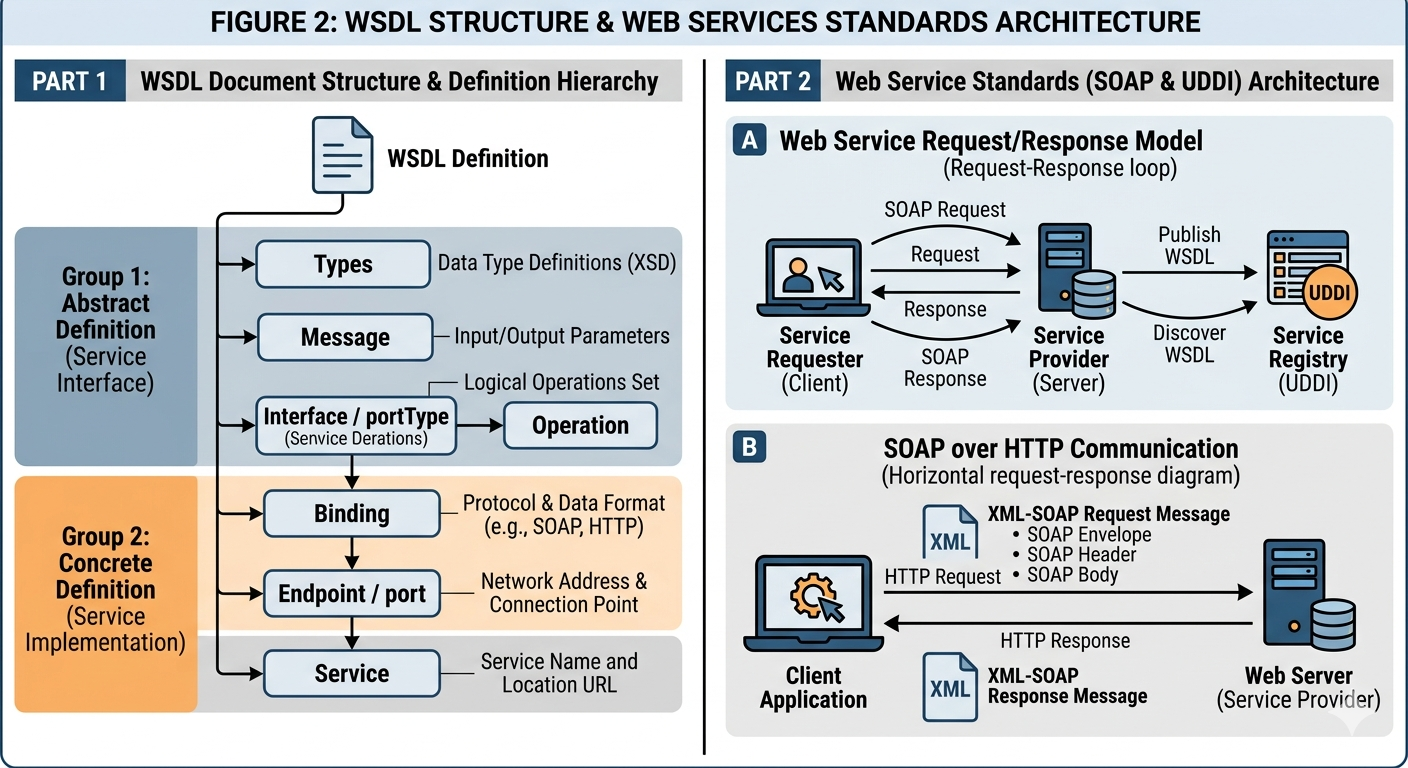
\includegraphics[width=1.0\textwidth]{pictures/wsdl.png}
    \caption{Структура на техническото WSDL описание (вляво) и архитектурна топология на SOAP/UDDI интеграцията (вдясно)}
    \label{fig:wsdl_soap}
\end{figure}

На Фиг. \ref{fig:wsdl_soap} подробно са декомпозирани стандартите за уеб услуги:
\begin{itemize}
    \item \textbf{Вляво (PART 1):} Йерархичната структура на WSDL документа. Тя строго разделя уеб услугата на \textbf{абстрактна част} (дефинираща логическия интерфейс чрез \textit{Types}, \textit{Message} и набора от операции — \textit{Interface / portType}) и \textbf{конкретна част} (описваща физическата имплементация чрез транспортния протокол \textit{Binding}, мрежовия адрес \textit{Endpoint / port} и крайната точка \textit{Service}).
    \item \textbf{Вдясно (PART 2):} Интеграционната топология и съобщителният модел. 
\end{itemize}

Секция \textbf{PART 2 (A)} илюстрира класическия трикомпонентен модел (Service Triangle). Важно е да се отбележи логическият поток на откриване на услуги: доставчикът (\textit{Service Provider}) публикува техническото WSDL описание в споделения UDDI регистър (\textit{Publish WSDL}). От своя страна, клиентът (\textit{Service Requester}) се обръща към UDDI регистъра, за да открие и свали съответния WSDL контракт (\textit{Discover WSDL}), след което инициира директна комуникация със сървъра.

В секция \textbf{PART 2 (B)} е показан самият транспорт на съобщенията. Комуникацията се осъществява по модела заявка-отговор (\textit{Request-Response loop}) над приложния протокол HTTP. Данните се капсулират в строго дефинирани XML-SOAP съобщения, чиято структура задължително съдържа коренов елемент \textit{SOAP Envelope}, метаданни в \textit{SOAP Header} и приложен товар в \textit{SOAP Body}.

\subsubsection{1. SOAP (Simple Object Access Protocol)}
SOAP е протокол за съобщения, имплементиран над HTTP или SMTP, целящ размяна на структурирана информация под формата на \textbf{XML обекти}. SOAP комуникацията (виж Фиг. \ref{fig:wsdl_soap}, вдясно) винаги се осъществява чрез HTTP заявки и отговори.

SOAP дефинира три задължителни елемента в своята спецификация:
\begin{itemize}
    \item \textbf{Envelope (Плик):} Кореновият XML елемент, който дефинира документа като SOAP съобщение.
    \item \textbf{Header (Хедър):} Опционален елемент, съдържащ метаданни (сигурност, маршрутизация, транзакции).
    \item \textbf{Body (Тяло):} Задължителен елемент, съдържащ реалните данни на заявката или отговора.
\end{itemize}

SOAP поддържа строго типизиран контракт, транзакции (WS-AtomicTransaction) и сигурност (WS-Security), което го прави подходящ за enterprise среди.

\subsubsection{2. WSDL (Web Service Description Language)}
WSDL е базиран на XML технически език, който специфицира интерфейса на дадена уеб услуга и детайлите за комуникация с нея. Той служи като допълнение към SOAP. Структурата на WSDL документа (Фиг. \ref{fig:wsdl_soap}, вляво) е разделена на:
\begin{itemize}
    \item \textbf{Абстрактна част (Abstract Definition):} Дефинира логическите интерфейси. Те включват типовете данни (\textit{Types}), структурата на съобщенията (\textit{Message}) и предлаганите операции (\textit{Interfaces / portTypes}).
    \item \textbf{Конкретна част (Concrete Definition):} Специфицира физическата имплементация. Тя описва обвързването към транспортен протокол (\textit{Bindings}), точната крайна точка (\textit{Endpoints / ports}) и конкретното мрежово местоположение на услугата (\textit{Services}).
\end{itemize}

\subsubsection{3. UDDI (Universal Description, Discovery, and Integration)}
UDDI е разпределена директорийна услуга (регистър), действаща като "телефонен указател" за бизнеса. Тя позволява на организациите да публикуват своите уеб услуги (описани чрез WSDL), а на клиентите — да ги откриват динамично.

UDDI архитектурно се състои от три логически компонента:
\begin{itemize}
    \item \textbf{Бели страници (White Pages):} Съдържат базова бизнес информация за доставчика на услугата (име, адрес, контакт).
    \item \textbf{Жълти страници (Yellow Pages):} Използват се за индустриална и стандартизирана класификация на предлаганите услуги.
    \item \textbf{Зелени страници (Green Pages):} Съдържат детайлната техническа и имплементационна информация за уеб услугите и начините за интеграция с тях.
\end{itemize}

\subsection{Message Brokers (опашки за съобщения)}
Message broker-ите осигуряват \textbf{асинхронен} обмен на съобщения между компонентите на разпределените системи. Издателят изпраща съобщение до брокера, а консуматорът го получава когато е готов — двата компонента не трябва да са активни едновременно.

Основни функции на message broker-ите:
\begin{itemize}
    \item \textbf{Буфериране:} Съобщенията се съхраняват до тяхната обработка.
    \item \textbf{Маршрутизиране:} По тематичен принцип (topic-based) или базирано на съдържанието (content-based).
    \item \textbf{Гарантирана доставка:} Поддържат се семантики като exactly-once и at-least-once.
    \item \textbf{Мащабируемост:} Разпределени опашки при голям товар.
\end{itemize}

\textbf{Примери за message broker-и:}
\begin{itemize}
    \item \textbf{Apache Kafka:} Log-базиран, с висока производителност и пропускателна способност.
    \item \textbf{RabbitMQ:} Базиран на AMQP протокола.
    \item \textbf{Apache ActiveMQ} и \textbf{AWS SQS}.
\end{itemize}

\subsection{Сравнение: RMI срещу Уеб услуги (SOAP/WSDL)}

\textbf{Прилики:} И двата модела се базират на протокола заявка-отговор (\textit{Request-Response}), целят пълна прозрачност за клиента и прилагат строго разделение на слоеве, за да скрият детайлите по мрежовия пренос от разработчика.

\textbf{Разлики:}
\begin{itemize}
    \item \textbf{Технологична обвързаност:} RMI е силно специализирано решение (обикновено за Java), докато SOAP/WSDL са напълно хетерогенни — независими от езика и платформата.
    \item \textbf{Откриване на услуги:} RMI разчита на лек RMI Registry, докато уеб услугите ползват мащабната UDDI директория (бели, жълти и зелени страници).
    \item \textbf{Формат на данните:} RMI използва двоична сериализация на Java обекти, докато SOAP предава структуриран XML, капсулиран в HTTP/SMTP плик.
\end{itemize}

\end{FlushLeft}

\end{document}
